\chapter*{The Procurator of Judea}

I think now would be a good time to turn to the problem of Pilate. From all that we know about him, it would seem that the ``cruel procurator of Judea, the equestrian Pontius Pilate''\footnote{\emph{The Master and Margarita}, p. 335 (with slight alteration)} was not so much incredibly cruel as he was absolutely heartless. So just what was it that twice compelled him to return to the case of a poor street preacher accused of \emph{crimen læse majestatis} (insulting royalty) and, instead of having him immediately executed---just ``for simplicity's sake,'' so to speak---do almost everything in his power to save him?

In an attempt to somehow explain Pilate's strange affection for Christ, Matthew the Evangelist cites the intercession of the procurator's wife, who supposedly had a relevant vision in a dream. Hold on---what wife is \emph{he} talking about? Still, let's suppose that the procurator really was married, and that he saw his wife's opinions on state affairs as anything more than hot air. What was she doing in Jerusalem, then?

The problem is that the procurators of Judea maintained a permanent residence in the seaside city of Caesarea, and Pilate only came to Jerusalem several times a year to oversee the collection of taxes and preside over trials.\footnote{``Pilate,'' \emph{Bible Encyclopedia} of Archimandrite Nicephorus, III:122} But perhaps she could have sent a messenger to her husband from their residence in Caesarea? Alas, that doesn't work either; the trial took place in the morning, his wife said that she ``suffered many things \emph{that day} in a dream because of Him'' (Mt 27:19), and the distance from Caesarea to Jerusalem is around 120 kilometers as the crow flies. And yet, this rumor (for it can be nothing but a rumor) about the role of Pilate's wife in this affair, which Matthew faithfully reproduced in his Gospel, is actually quite important. Let's keep it in the back of our minds for now.

With regard to Bulgakov's stunning reconstruction, it suffers, in my opinion, from only one flaw: his Pilate is too human. Not in the sense of being ``too humane,'' but of being too susceptible to normal human emotions: curiosity, affinity and hostility, loneliness, and of course, cowardice (``the most terrible vice,''\footnote{\emph{The Master and Margarita}, p. 272.} as the procurator himself admits). In this sense, Dombrovsky's Pilate, a high-ranking imperial apparatchik, seems far more true to life:

\begin{smallquote}
    ``Hence Pilate's initial hesitation. He simply didn't want to execute anyone for the benefit of the Jews. But there was a second consideration. Reasons of state this time. The fact of the matter was that Christ, or someone like him, suited Pilate's book very well. Surprised? It's quite simple really. He had thoroughly assimilated two aspects of Christ's teaching. In the first place, this wandering preacher did not believe either in war or revolutionary upheaval; no, man must refashion himself from within, and then everything would happen by itself. Therefore he was against rebellion. That was the first point. Second: the only thing Jesus that sought to destroy and actually was undermining all the time, were the authorities. The authority of the sanhedrin, the Sadducees and the Pharisees, and so, perhaps unwittingly, the authority of Moses and the temple. And it was in the monolithic and unquestionable nature of these that the greatest danger to the Empire resided. Clearly Rome needed precisely the sort of subversion that Jesus represented. [...] Now imagine the state of the world at that time and ask yourself whether or not such utterances in the mouth of the Galilean did not suit Pilate? Didn't it mean a prescription to pray for and love him, the occupier? Surely Pilate, a state official who knew the East and the land he was attempting to pacify, realized that this was the very force on which he ought to rely?''\footnote{\emph{The Faculty of Useless Knowledge,}, trans. Alan Myers, pp. 290-291.}
\end{smallquote}

I included such a lengthy quote simply because these generally surface-level considerations often paradoxically go unnoticed. It seems that whenever the relationship between the Roman authorities and early Christianity comes up, people immediately think back to the tar-covered human torches of Nero's reign, as well as other equally colorful incidents. Be that as it may, what we are talking about here is another time and another place, and politics, as Churchill once famously said, sometimes makes for strange bedfellows.

You can argue all you want against early Christianity's assessment as a peace-loving doctrine by citing verses such as ``I did not come to bring peace, but a sword'' (Mt 10:34) and other, equally noteworthy passages from Holy Scripture. The fact remains, however: thirty years later, members of the first Christian communities actually refrained from taking part in the Great Revolt and the Jewish War, for which their fellow countrymen branded them as Roman collaborators and exiled them to Transjordan. So if Pilate's attempts to save Jesus really were motivated by the aforementioned considerations of state, he was certainly right on the money. As for the long-term consequences, the procurator---honest to God!---had far more important things to worry about than someone else's future headache.

% [htbp]: Instructs LaTeX to try placing the image Here, at the Top, Bottom, or on a separate Page (in that order).
\begin{figure}[htbp]
    \centering
    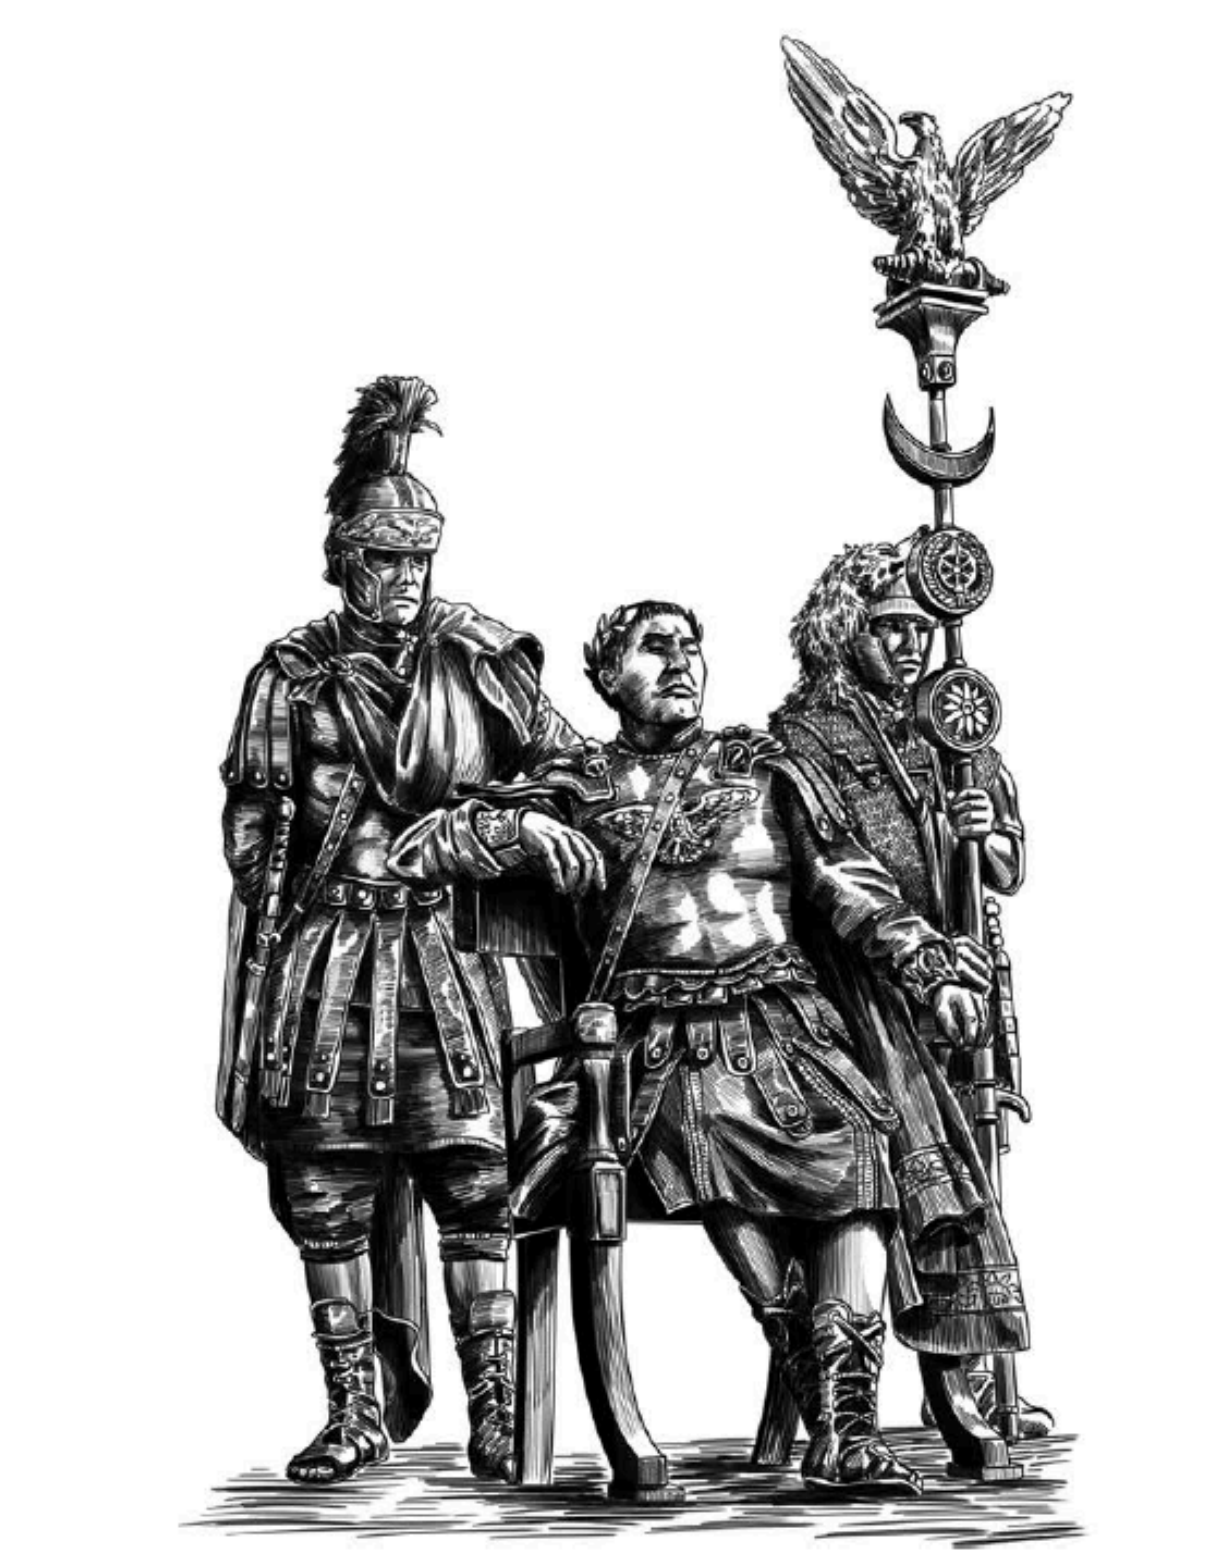
\includegraphics[width=0.5\textwidth]{assets/procurator.png}
    % \caption{The Procurator of Judea}
    \label{fig:pilate}
\end{figure}

So that's why he \emph{tried} to save Jesus. But why \emph{didn't} he? Why, after stating his premise (be it for reasons of state, to spite his enemies in the Sanhedrin, or simply on a lordly whim), did he not follow through to its conclusion and use his vast range of powers to their fullest extent? The standard version---``he chickened out because the local muckamucks threatened to snitch on him to the Dear Leader''---doesn't sound even remotely convincing. By that time, they had burned all possible bridges with the local authorities; a report here, a report there, what difference could it make?

Besides, an administrator as experienced as Pilate surely knew that such an accusation was never the actual reason for any punitive action; it could only ever be used as a formal pretext, if your fate was already sealed regardless. On the other hand, the procurator had already engaged in misconduct the moment he \emph{attempted} to exonerate a ``state criminal''; had this attempt been successful, that hardly would have mattered from the point of view of Tiberius' totalitarian regime (in the event they brought it to trial). Thus, so long as we assume that the driving force behind \emph{our} Pilate's actions were serious considerations of state, we can look at his ``about-face'' in that light as well.

Now, let us turn our attention to a rather significant detail, which for some reason, commentators on the Bible always seem to miss (or intentionally ignore). It is common knowledge that Christian tradition has done all it can to vindicate Pilate (in the Coptic and the Ethiopian Churches, he has even been canonized), laying all the blame for Christ's tragic death on the Jews. Meanwhile, in the time between Pilate's two ``not guilty'' verdicts, another was rendered: that of Herod Antipas, the Tetrarch (King) of Galilee. This detail, when considered with respect to the traditional view, is nothing short of outrageous. Let me explain.

As the representative of the semi-legitimate Idumean Dynasty, it was Herod, not the Sanhedrin, whose interests were most greatly affected by the crime Jesus was charged with---pretending to the Judean throne (``Are you the King of the Jews?''). Nevertheless, the Sanhedrin stubbornly insisted that Jesus be executed, and Herod, just like Pilate, saw absolutely nothing criminal in his actions. And this was the very same Herod who could be accused of everything except the ``idiotic disease of complacency'':\footnote{A phrase originating from one of Stalin's decrees, in which he alleged that several (mostly Jewish) doctors had conspired to assassinate government officials by way of ``negligence''; in context, it was used to lambaste the security services' purported inability to thwart the conspiracy. (Z.B.)} the platter with John the Baptist's head is more than enough evidence of that.

And in fact, no ruler, being of sound mind and body, would willingly prevent
the execution of a dubious prophet; either he is mad, or he is a rebel. As the khan
in \emph{The Enchanted Prince} tells his vizier in a similar situation:

\begin{smallquote}
    ``Once he has been seized and thrown into prison, why not cut his head off for safety's sake? We see no reasonable cause for abstaining! Revolt is much more serious than those Peshawar sorceries of yours, it is no joking matter!''\footnote{\emph{The Enchanted Prince}, Leonid Solovyov, trans. Bernard Isaacs, p. 167.}
\end{smallquote}

The explanation Christian commentators give for this usually runs along the lines of, ``Christ's innocence was so obvious that even a man as cruel and debauched as Herod could not uphold the Sanhedrin's verdict.''\footnote{ Universally Accessible Interpretation of the Gospel.} However, that is nothing more than childish prattle; in such situations, one's actual guilt or innocence means absolutely nothing. For Herod not to have subjected Jesus to the same \emph{Precautions} discussed by the aforementioned khan, he must have been under some degree of pressure, the source of which is quite obvious. Thus, Pilate's efforts to save Jesus must have been even more serious and sustained than the Gospel texts directly imply.

Herod's position (whether it was arrived at independently or by force), which is typically ignored as an insignificant detail, actually changes the picture of the balance of power quite radically. The image of an austere, honest Roman official, alone in his opposition to the Jews and their unshakeable religious fanaticism, disappears. In its place appear two supreme authorities---one Roman, one Jewish---who find themselves pestered by the ridiculous claims of one of the Judean public bodies. I should point out that the Sanhedrin functioned as not a criminal, but a purely religious tribunal, and the case they brought before Pilate was not even remotely within their jurisdiction. The Sanhedrin had full right to declare Christ a blasphemer and a heretic posing as the Son of God, and on those grounds they could sentence him to \emph{stoning} once they had submitted their---religious---verdict to the procurator for his purely formal approval.\footnote{ It was to stoning, the method of execution imposed for crimes against the Faith, that the high priest Ananus went on to sentence James, brother of Jesus several years later---without even bothering to inform the Roman procurator (Antiquities of the Jews, Book XX, 9:1). (K.E.)} Instead, with a persistence that remains completely incomprehensible, they slap the heretic Christ with trumped-up political charges and demand that Pilate \emph{crucify} him as a political criminal---a pretender to the Judean throne. As a result, the Sanhedrin, who have lacked the requisite authority from the very beginning, have moreover taken a legally indefensible position in their opposition to the secular authorities (namely, Pilate and Herod). And yet, at the very moment when it seems his opponent has no cards left to play, not even the very worst one, Pilate suddenly and inexplicably capitulates. What's the deal here?

The deal was that 23 relatively smart members of the Jewish clergy understood Christ's teachings just as well as Pilate did, and realized the threat posed by the young prophet's continued growth in popularity---both to the Temple of the Jewish faith and to them personally. And with that knowledge, they made a counterintuitive yet, as it turned out, perfectly calculated move: they arrested Jesus and came to Pilate with a blatantly illegal request---to execute him as a political criminal. This resulted in a magnificent ``fork'': either their hated rival would be liquidated at the hands of the Romans (with time, he could even be canonized asyet another hero who died at the occupiers' hands), or the procurator would let him go free, thereby acknowledging that the notorious Christ was a Roman ``agent of influence'' and rendering the prophet a political corpse.

There are serious grounds to believe that the Sanhedrin found the second option far more desirable, and more likely. Recall that if the high priests' only goal was to have Christ's head, then it would have been far simpler to go with the foolproof option of rendering a religious verdict. In any case, Pilate's approval of the execution of the ``King of the Jews'' clearly took them by surprise---kind of like someone who theatrically asks for his dismissal, then actually gets it. Only pure bewilderment could explain their panicked request for a Roman guard to patrol the burial site---this, in a city chock full of temple guards!

...The procurator realized he had lost: it was useless to keep up the fight for Jesus. Of course, he could simply pardon the Galilean, stamping a big fat X on his viability as a political figure, but that would just be pure capitulation. Nonetheless, he could still try to derive some benefit from the death of the popular prophet (as a benefit in this case meant anything to the Sanhedrin's detriment). And so, after making a show of washing his hands, Pilate---entirely of his own accord!---hands Jesus over to the soldiers for torture, then demonstrates to the crowd: it is the Sanhedrin that is guilty. From this moment on, the Sanhedrin will be guilty of everything, down to the gall and sour wine Christ is given by Roman soldiers (Mt 27:34). I've got to hand it to him---despite being down a piece, Pilate ultimately won the initiative and, to some extent, managed to equalize the game. The persistence and ingenuity of this ruthless chessmaster are certainly worthy of respect, but as for what could have possibly led anyone to canonize him, I admit I haven't the slightest idea.

But still, was there really no way for Pilate to even theoretically save Jesus, without ``outing'' him? Yes, there was---and he didn't hesitate to use it. ``At the feast the governor was accustomed to releasing to the multitude one prisoner whom they wished'' (Mt 27:15); so really, if the crowd in the square picked Jesus, the procurator could have released him without any problem, as there would be no sign of a ``Roman trail.'' But luck was not on his side; the crowd, of course, chose Barabbas---it would be strange if the high priests were careless and failed to ensure that the ``voice of the people'' was duly trained. However, this---completely natural---choice on the part of the Jews comes as a total surprise to Pilate. He repeats his request three times, entering into a pointless bickering match with the crowd that only leaves him further humiliated---in other words, he completely loses face.

So, the \emph{natural} course of events has clearly caught the procurator off guard. From this, it is logical to assume that there was some factor unknown to us (but known to the procurator) that was supposed to interfere with the natural course of events. \emph{Supposed} to, but didn't. The ``million dollar question'': what was this factor, and why didn't it work out as planned?